%%% DOCUMENTCLASS 
%%%-------------------------------------------------------------------------------

\documentclass[
a4paper, % Stock and paper size.
11pt, % Type size.
% article,
% oneside, 
onecolumn, % Only one column of text on a page.
openright, % Each chapter will start on a recto page.
% openleft, % Each chapter will start on a verso page.
%openany, % A chapter may start on either a recto or verso page.
]{memoir}

%%% PACKAGES 
%%%------------------------------------------------------------------------------

\usepackage[utf8]{inputenc} % If utf8 encoding
% \usepackage[lantin1]{inputenc} % If not utf8 encoding, then this is probably the way to go
\usepackage[T1]{fontenc}    %
\usepackage{lmodern}
\usepackage[USenglish]{babel} % English please
\usepackage[final]{microtype} % Less badboxes
\usepackage{float}
% \usepackage{kpfonts} %Font

\usepackage{amsmath,amssymb,mathtools} % Math

% \usepackage{tikz} % Figures
\usepackage{graphicx} % Include figures

%%% PAGE LAYOUT 
%%%------------------------------------------------------------------------------

\setlrmarginsandblock{0.15\paperwidth}{*}{1} % Left and right margin
\setulmarginsandblock{0.2\paperwidth}{*}{1}  % Upper and lower margin
\checkandfixthelayout

%%% SECTIONAL DIVISIONS
%%%------------------------------------------------------------------------------

\maxsecnumdepth{subsection} % Subsections (and higher) are numbered
\setsecnumdepth{subsection}

\makeatletter %
\makechapterstyle{standard}{
  \setlength{\beforechapskip}{0\baselineskip}
  \setlength{\midchapskip}{1\baselineskip}
  \setlength{\afterchapskip}{8\baselineskip}
  \renewcommand{\chapterheadstart}{\vspace*{\beforechapskip}}
  \renewcommand{\chapnamefont}{\centering\normalfont\Large}
  \renewcommand{\printchaptername}{\chapnamefont \@chapapp}
  \renewcommand{\chapternamenum}{\space}
  \renewcommand{\chapnumfont}{\normalfont\Large}
  \renewcommand{\printchapternum}{\chapnumfont \thechapter}
  \renewcommand{\afterchapternum}{\par\nobreak\vskip \midchapskip}
  \renewcommand{\printchapternonum}{\vspace*{\midchapskip}\vspace*{5mm}}
  \renewcommand{\chaptitlefont}{\centering\bfseries\LARGE}
  \renewcommand{\printchaptertitle}[1]{\chaptitlefont ##1}
  \renewcommand{\afterchaptertitle}{\par\nobreak\vskip \afterchapskip}
}
\makeatother

\chapterstyle{standard}

\setsecheadstyle{\normalfont\large\bfseries}
\setsubsecheadstyle{\normalfont\normalsize\bfseries}
\setparaheadstyle{\normalfont\normalsize\bfseries}
\setparaindent{0pt}\setafterparaskip{0pt}
\setlength{\parskip}{1em}

%%% FLOATS AND CAPTIONS
%%%------------------------------------------------------------------------------

\makeatletter                  % You do not need to write [htpb] all the time
\renewcommand\fps@figure{htbp} %
\renewcommand\fps@table{htbp}  %
\makeatother                   %

\captiondelim{\space } % A space between caption name and text
\captionnamefont{\small\bfseries} % Font of the caption name
\captiontitlefont{\small\normalfont} % Font of the caption text

\changecaptionwidth          % Change the width of the caption
\captionwidth{1\textwidth} %

%%% ABSTRACT
%%%------------------------------------------------------------------------------

\renewcommand{\abstractnamefont}{\normalfont\small\bfseries} % Font of abstract title
\setlength{\absleftindent}{0.1\textwidth} % Width of abstract
\setlength{\absrightindent}{\absleftindent}

%%% HEADER AND FOOTER 
%%%------------------------------------------------------------------------------

\makepagestyle{standard} % Make standard pagestyle

\makeatletter                 % Define standard pagestyle
\makeevenfoot{standard}{}{}{} %
\makeoddfoot{standard}{}{}{}  %
\makeevenhead{standard}{\bfseries\thepage\normalfont\qquad\small\leftmark}{}{}
\makeoddhead{standard}{}{}{\small\rightmark\qquad\bfseries\thepage}
% \makeheadrule{standard}{\textwidth}{\normalrulethickness}
\makeatother                  %

\makeatletter
\makepsmarks{standard}{
\createmark{chapter}{both}{shownumber}{\@chapapp\ }{ \quad }
\createmark{section}{right}{shownumber}{}{ \quad }
\createplainmark{toc}{both}{\contentsname}
\createplainmark{lof}{both}{\listfigurename}
\createplainmark{lot}{both}{\listtablename}
\createplainmark{bib}{both}{\bibname}
\createplainmark{index}{both}{\indexname}
\createplainmark{glossary}{both}{\glossaryname}
}
\makeatother                               %

\makepagestyle{chap} % Make new chapter pagestyle

\makeatletter
\makeevenfoot{chap}{}{\small\bfseries\thepage}{} % Define new chapter pagestyle
\makeoddfoot{chap}{}{\small\bfseries\thepage}{}  %
\makeevenhead{chap}{}{}{}   %
\makeoddhead{chap}{}{}{}    %
% \makeheadrule{chap}{\textwidth}{\normalrulethickness}
\makeatother

\nouppercaseheads
\pagestyle{standard}               % Choosing pagestyle and chapter pagestyle
\aliaspagestyle{chapter}{chap} %

%%% NEW COMMANDS
%%%------------------------------------------------------------------------------

\newcommand{\p}{\partial} %Partial
% Or what ever you want

\graphicspath{{Figuren/}} 

%%% TABLE OF CONTENTS
%%%------------------------------------------------------------------------------

\maxtocdepth{subsection} % Only parts, chapters and sections in the table of contents
\settocdepth{subsection}

\AtEndDocument{\addtocontents{toc}{\par}} % Add a \par to the end of the TOC

%%% INTERNAL HYPERLINKS
%%%-------------------------------------------------------------------------------

\usepackage{hyperref}   % Internal hyperlinks
\hypersetup{
pdfborder={0 0 0},      % No borders around internal hyperlinks
pdfauthor={I am the Author} % author
}
\usepackage{memhfixc}   %

%%% THE DOCUMENT
%%% Where all the important stuff is included!
%%%-------------------------------------------------------------------------------

\author{Friedl De Groote, Maarten Afschrift, Jente Willaert}
\title{Direct collocation tutorial}


\begin{document}

\frontmatter

\maketitle

%\begin{abstract}

%\end{abstract}
\clearpage

\tableofcontents*
\clearpage

\mainmatter

\chapter{Dynamics of the pendulum test}

In this tutorial, we use the pendulum test for spasticity \cite{degroote2018} as an example to illustrate numerical simulations of movement, and the use of direct collocation to solve optimal parameter estimation and optimal control problems. 

The pendulum test has been shown to be sensitive to the presence and severity of spasticity. While the patient is seated, the examiner drops the lower leg from the horizontal position, with the knee joint extended; the lower leg is then allowed to swing freely under the influence of gravity and joint kinematics are recorded.

We describe the dynamics of the lower leg during the pendulum test based on a torque-driven biomechanical model (Figure \ref{Fig:model}). The model consists of a planar lower leg segment with passive stiffness and damping to simulate non-contractile musculotendon properties. Active joint torques representing muscle contractile behavior consist of a constant baseline torque to represent muscle tone, 
% a short-range stiffness torque dependent on the level of muscle tone, 
and a delayed sensory feedback torque to simulate reflex activity (Figure \ref{Fig:model}).  
% Muscle short-range stiffness was scaled as a function of muscle tone. We simulated the reflex contributions to the pendulum test by modeling sensory feedback pathways based on either joint position and velocity to represent muscle length and velocity, or active torque and derivative of active torque to represent muscle fiber force and derivative of force. All model parameter values were held constant over the time course of each simulation.

\begin{figure}
  \begin{center}
    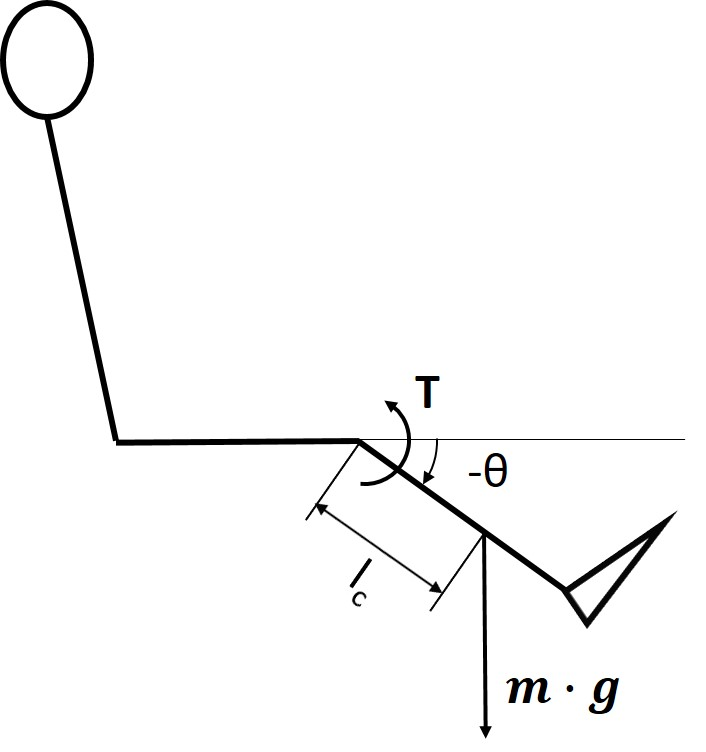
\includegraphics[width=0.4\textwidth]{Figure1.jpg}
  \end{center}
  \caption{Pendulum test model.}
  \label{Fig:model}
\end{figure}

%Our model consists of a planar lower leg segment actuated with a passive torque representing non-contractile musculotendon properties, Tpas, and an active torque representing muscle contractile behavior, Tact. 
Let us first consider a healthy subject in which reflex activity is absent. In that case, only gravity, damping and a constant baseline tone act on the lower leg. Knee joint motion is described by the equation of motion of the planar lower leg segment under the assumption that the knee joint center is stationary during the test:
\begin{equation}
% I \ddot{\theta} = m g l_c cos(\theta) - T_b - B \dot{\theta},
I \frac{d^2\theta(t)}{dt^2} = m g l_c cos\theta(t) - T_b - B \frac{d\theta(t)}{dt},
\label{eqofmot}
\end{equation}
where $t$ is time, $\theta$ is the knee joint angle ($\theta = 0$ corresponds to full extension and negative values correspond to knee flexion), $I$ is the moment of inertia of the lower leg with respect to the knee, $m$ is the mass of the lower leg, $g$ is gravitational acceleration, and $l_c$ is the distance between the knee joint center and the center of mass of the lower leg (Figure xx). 
% Note that we use $\dot{\theta}$ and $\ddot{\theta}$ as short notations for respectively $\frac{d\theta}{dt}$ and $\frac{d^2\theta}{dt^2}$.

The movement of the lower leg is described by a second order differential equation (\ref{eqofmot}), i.e., the second (but not the third or any higher) derivative of the knee angle with respect to time appears in the equation. Hence, the movement of the lower leg can be described by two states: knee joint angle $\theta$ and knee joint angular velocity $\dot{\theta}$, where $\dot{\theta}$ is short notation for $\frac{d\theta}{dt}$. And based on (\ref{eqofmot}) we can write explicit equations for the state derivatives:
\begin{eqnarray}
% J \ddot{\theta} = m g l_c cos(\theta) - T_b - B \dot{\theta},
\frac{d\theta(t)}{dt} & = & \dot{\theta}(t), \label{eqofmot1}\\
\frac{d \dot{\theta}(t)}{dt} & = &\frac{1}{I} \left( m g l_c cos\theta(t) - T_b - B \dot{\theta}(t) \right).
\label{eqofmot2}
\end{eqnarray}


\chapter{Forward simulations}

Based on the equations of motion (equations \ref{eqofmot1}-\ref{eqofmot2}) we can numerically simulate the lower leg movement if we know the initial state, i.e., the knee joint angle $\theta_0$ and angular velocity $\dot{\theta}_0$ at $t = 0$. 

To this aim, we discretize the states. Or in other words, we represent the continuous states, $\theta(t)$ and $\dot\theta(t)$, over a time interval $[t_0 \: t_f]$ by a finite number of values representing the state at discrete time instants $i$: $[\theta_0 \: \theta_1 \: \ldots \: \theta_i \: \ldots \: \theta_N]$ and $[\dot\theta_0 \: \dot\theta_1 \: \ldots \: \dot\theta_i \: \dot\ldots \: \dot\theta_N]$. For simplicity, let us consider $N + 1$ equidistant time instants. In that case, the time between consecutive time instants $\Delta t$ is constant and equals $\frac{t_f - t_0}{N}$. 

Next, we approximate the exact time derivatives by numerical derivatives. Using a simple backward backward Euler scheme results in:
\begin{eqnarray}
\frac{d\theta_i}{dt} & \approx & \frac{\theta_{i+1} - \theta_{i}}{\Delta t}, \\
\frac{d\dot\theta_i}{dt} & \approx & \frac{\dot\theta_{i+1} - \dot\theta_{i}}{\Delta t}.
\label{BE}
\end{eqnarray}
Using these approximations for the derivatives, we can now discretize the dynamic equations \ref{eqofmot1}-\ref{eqofmot2}:
\begin{eqnarray}
\frac{\theta_{i+1} - \theta_{i}}{\Delta t} & = & \dot{\theta_i}, \\
\frac{\dot\theta_{i+1} - \dot\theta_{i}}{\Delta t} & = &\frac{1}{I} \left( m g l_c cos\theta_i - T_b - B \dot{\theta}_i \right).
\label{discseteqofmot}
\end{eqnarray}
We can solve these equations for $\theta_{i+1}$ and $\dot\theta_{i+1}$:
\begin{eqnarray}
\theta_{i+1} & = & \theta_{i} + \dot{\theta_i} \Delta t , \label{expdisceqofmot1}\\
\dot\theta_{i+1} & = & \dot\theta_{i} + \frac{\Delta t}{I} \left( m g l_c cos\theta_i - T_b - B \dot{\theta}_i \right).
\label{expdisceqofmot2}
\end{eqnarray}
Starting from the given initial states $\theta_0$ and $\dot{\theta}_0$, we can iteratively solve equations \ref{expdisceqofmot1}-\ref{expdisceqofmot2} to find the states at times $1 \ldots N$. Such procedure for numerical integration is often referred to as time marching, since the discrete states at consecutive time instants are iteratively computed. For an implementation, see Part2\_Discretization.m (section Part 2A).

The use of variable instead of fixed time steps and more accurate discretization schemes than backward Euler can improve numerical accuracy of the integration. Matlab provides different solvers for numerical integration of ordinary differential equations (e.g., equations \ref{eqofmot1}-\ref{eqofmot2}). For an example implementation using ode23, see Part2\_Discretization.m (section Part 2C).

Alternatively, we can insert the approximations for the derivatives directly in equation \ref{eqofmot} after bringing all the terms to the left hand side of the equation:
\begin{equation}
I \frac{\dot\theta_{i+1} - \dot\theta_{i}}{\Delta t} - m g l_c cos\theta(t) + T_b + B \frac{\theta_{i+1} - \theta_{i}}{\Delta t} = 0.
\label{disceqofmot}
\end{equation}
Equations \ref{expdisceqofmot1} and \ref{disceqofmot} for $i = 1 \ldots N$ form a set of equations that can be solve numerically, e.g. by using fsolve in matlab, for $\theta_i$ and $\dot{\theta}_i$ if the initial states $\theta_0$ and $\dot{\theta}_0$ are known.  
For an implementation, see Part2\_Discretization.m (section Part 2B).
As opposed to time marching forward integration, here all discrete states are simultaneously computed. % Maybe note on numerical condition. 


\chapter{Controller}

To do.

\chapter{Optimal parameter estimation and optimal control}

Here, we discuss different numerical approaches to find the values for the baseline torque $T_b$ and damping $B$ that result in simulated knee angle trajectories that best match experimental knee angle trajectories. 

Finding the model parameters $T_b$ and $B$ that result in the best agreement between measured and simulated knee angle trajectories requires solving a dynamic optimization problem. The agreement between measured and simulated knee angle trajectories can be described by
\begin{equation}
J = \sum_{i = 1}^{N} ( \theta_i - \hat{\theta}_i )^2,
\end{equation}
where $\theta_i$ and $\hat{\theta}_i$ are respectively simulated and experimental joint angle at time instant $i$. Hence, the corresponding optimization problem is to minimize the cost function $J$ with respect to optimization variables $ p = [T_b \: B]$. 

\section{Direct shooting}

Shooting methods evaluate the cost function $J$ by using time marching forward integration to solve for $\theta_i$. Gradient based optimization methods typically require many function evaluations to obtain derivative information through finite differences. Hence, in every iteration of the optimization algorithm the dynamics are evaluated multiple times through forward integration. 

To obtain accurate approximations of the derivatives through finite differences, it is important that the same numerical operations are performed when evaluating $J(p)$ and $J(p+\Delta p)$. In this case, this means that the discretization scheme used by the integrator should be the same. For an example implementation using Matlab's fmincon see Part4\_Shooting\_Fmincon.m.

Shooting methods are not very well suited for systems with stiff dynamics, where the simulated state trajectories have a high sensitivity to the optimization variables. Typically, this sensitivity increases with simulation time.

\section{Direct collocation}

In contrast to shooting methods, direct collocation methods do not rely on time-marching to evaluate the dynamics. Instead, the discretized states are considered as additional optimization variables and the discretized state equations \ref{expdisceqofmot1} and \ref{disceqofmot} are imposed as constraints. This results in a non-linear programming problem with a large number of optimization variables and constraints as compared to direct shooting. However, the sparsity of the resulting optimization problems makes them tractable. By reducing the sensitivity of the cost function to the optimization variables, direct collocation methods are often numerically more efficient than shooting methods. Note that the dynamic equations do not need to be satisfied in every iteration of the optimization algorithm when using direct collocation. 

For an example implementation using Matlab's fmincon see Part4a\_DirectCollocation  \_Fmincon.m. By exploiting sparsity and by using algorithmic differentiation, numerical efficiency can be improved. For example implementations using CasADi (www.casadi.org) see Part4b\_DirectCollocation\_Casadi.m and Part4a\_DirectCollocation\_Casadi\_Opti.m.


\chapter{Hands-on tutorial}


% Part_Input.m
% explain pendulum test with figure

% Part2_Discretization


\begin{thebibliography}{9}
\bibitem{degroote2018} 
De Groote, F., Blum, K.B., Horslen, B.C., Ting, L.H. Interaction between muscle tone, short-range stiffness and increased sensory feedback gains explains key kinematic features of the pendulum test in spastic cerebral palsy: A simulation study. 
\textit{PLoS ONE}, 13(10):e0205763, 2018. 
\end{thebibliography}

\end{document}